\chapter{Experimental design and Data exploration}
\label{ch:ExpDesign}

Ideally, you would like to design experiments (manipulations and/or 
observations) that are appropriate for the question you want to answer. 
However, you still need to explore you data to determine what kind of 
statistical tests would be appropriate because: (a) Your experiments or 
observations may not go as planned, and (b) You might have somebody 
else's data to analyse (very likely in your UG projects). Building on 
the previous chapter, in this chapter we you learn how to use R to 
explore your data and determine appropriate statistical tests. By the 
time you have worked through this chapter, you should be able to 

\begin{compactitem}
	\item Provided sufficient information is available, be able to judge 
	whether the sampling design used to generate a particular dataset was 
	appropriate
	\item Determine if your sample sizes are adequate, especially for a 
	specific statistical test qualitatively (Y1) or quantitatively using 
	power analysis (Y2). 
	\item Calculate basic statistical measures on your data to determine 
	its properties
\end{compactitem}

We are going to start off in Y1 with the simplest of scenarios for 
statistical testing --- that you want to determine whether a sample, or 
a pair of samples meet some expectation (hypothesis) or not. 

First, some conceptual preliminaries.

\section{Some statistical parlance}
The following terms are important for you to get familiar with:
\begin{description}
    
		\item[(Statistical) Population] A statistical population is a {\it 
		complete set} of items that share at least one {\it attribute} of 
		interest. This attribute of interest is the target of your 
		statistical analysis. For example, if we are interested in studying 
		the weight of year-old cod in the Oceans, the population 
		consists of {\it all} year-old cod, but more specifically, the 
		weight measurements of all the individuals of the cod population is 
		what we want to analyse. 
    
		\item[(Statistical) Distribution] A statistical distribution is a 
		mathematical description (expressed as a mathematical equation) of 
		the properties of a population of interest. Theoreticians have come 
		up with a bunch of distributions (e.g., Gaussian or Normal, 
		Poisson, Binomial, etc.) that are appropriate for different kinds 
		of data. Figuring out which distribution best describes a 
		population of interest is one of the first steps in a statistical 
		analysis. In reality, of course, even collecting and measuring all 
		the individuals of a population may not be sufficient to 
		characterize its statistical properties --- imagine the situation 
		where the cod population has declined to a few hundred individuals 
		(not an impossibility in the future!).
    
		\item[(Data or Population) Sample] A data {\it sample} is a set of 
		measurements of the attribute of interest collected from a {\it 
		statistical population} by a defined procedure ({\it sampling 
		methodology}). In the cod example above, this would be the weight 
		of every individual of a {\it subset} of the year-old Cod 
		population.

		\item[(Statistical) Parameter]  A statistical parameter is a 
		measure of some attribute of the {\it theoretical} statistical 
		distribution that is support to represent your population. An 
		example would be the average weight of yearling cod. In 
		practice, this is not measurable because the population is much too 
		large or incompletely inaccessible/invisible --- imagine measuring 
		the weight of every year-old cod individual in the oceans!   

		\item[Statistic] A statistic (singular) is an {\it estimate} of a 
		statistical parameter of the population of interest, obtained by 
		calculating the {\it measure} for a {\it sample} (e.g.,  the 
		average or mean weight of individuals in a sample of one-year old 
		cod). This is also your {\it descriptive statistic}. Therefore, a 
		{\it Statistic} is to a {\it Statistical Parameter} what a {\it 
		Sample} is to the {\it Statistical Population}. For example, the 
		average of a sample of cod weights is a statistic that {\it 
		estimates} the theoretical ``real'' average of the weights of the 
		entire one-year Cod population, which is its statistical parameter.
    
		\item[Hypothesis] A Hypothesis is an (hopefully) informed {\it 
		postulate} about an attribute of your population of interest. For 
		example, you may hypothesize that the one-year old cod population's 
		mean weight has declined over the last two decades (it has!). You 
		will want to confront your main hypothesis with a ``null'' 
		Hypothesis, to minimize the risk of making a ``type I'' error. A 
		type I error is the probability of accepting an alternative (or 
		main) hypothesis (and rejecting the null hypothesis) that is not 
		really valid (e.g., the yearling cods have actually not declined in 
		weight). This is a big NO NO from a scientific and philosophical 
		standpoint. The rate or probability of the type I error is denoted 
		by the Greek letter $\alpha$, and equals the {\it significance 
		level} of a statistical test.

\end{description}

\section{Descriptive Statistics}

The fundamental statistics that describe a sample (or a population) 
are, firstly, the mean, or average value of a sample, typically denoted 
by a $\bar{x}$: 

\begin{equation}
	\bar{x} =  \frac{\sum\limits_{i=1}^n x_i}{n} = \frac{x_{1} + x_{2} + \dots +x_{n}}{n}
\end{equation}

That is, it is the sum of all the values in a sample divided by the 
number, $n$, of items in the sample. Thus it is a measure of the {\it 
central-tendency} of the sample and population.

Second, the standard deviation ($s$) is:

\begin{equation}
	s =  \sqrt{\frac{\sum\limits_{i=1}^n (\bar{x} - x_{i})^2}{n-1}} = 
	\sqrt{\frac{(\bar{x} - x_{1})^{2} + (\bar{x} - x_{2})^2 + \dots + (\bar{x} 
	- x_{n})^{2}}{n-1}}
\end{equation}

That is, the the square root of the sum of squares ("SS") of the 
differences between each item in the sample and the mean, divided by 
the {\it degrees of freedom, "df"} remaining in the data set ($ 
n-1$). df is the sample size, $n$, minus the number of statistical 
parameters estimated from the data set. This is to reduce the {\it 
bias} in your {\it estimate} of the statistic, as you are calculating 
it from the sample, and not the whole theoretical population.

Thus, the formula for $s$ above has $n-1$ in its denominator because, 
to to work out the standard deviation, you must have already estimated 
the mean ($\bar{x}$) from the same data set. This removes 1 degree of 
freedom. Also, note that the sample variance, $s^2$ is the square of 
standard deviation. Or, in other words, the standard deviation is the 
square-root of the variance! 

The above two statistics (mean and sd) are particularly meaningful when 
the sample and population have a symmetric distribution (e.g., normal 
or gaussian). When the distribution is not symmetric (that is, it is 
{\it skewed}), another statistic, the {\it median} becomes important. 
This is the middle value in the ordered set of data, that is exactly 
50\% of the data live below and 50\% lie above the median. In skewed 
distributions, the median is a better measure of the 
{\it central-tendency} of the sample and population. 

Other descriptive statistics you should keep in mind are the range 
(difference between the largest and smallest values), and the quartiles 
(values lying in the data divided into the intervals $[{1\over4}, {1\over 
2},{3\over 4}, 1]$ or at 1\% intervals (percentiles). Box-plots, which 
you have seen, represent a number of these statistics in one figure.   

\subsection{Descriptive statistic functions in R}

\begin{tabular}{p{3.5cm} p{9.5cm}}
	{\tt mean(x)} & Compute mean (of a vector or matrix)\\
	{\tt sd(x)} & Standard deviation\\
	{\tt var(x)} & Variance\\
	{\tt median(x)} & Median\\
	{\tt quantile(x,0.05)} & Compute the 0.05 quantile\\
	{\tt range(x)} & Range of the data\\
	{\tt min(x)} & Minimum\\
	{\tt max(x)} & Maximum\\
	{\tt sum(x)} & Sum all elements\\
\end{tabular}\\

\section{Data types and distributions}
You will typically encounter or sample the following main types of 
data:

\begin{description}

		\item[Continuous numeric] This is the {\tt  numeric} or {\tt real} 
		data type in R, and as far as you are concerned, these data 
		typically will be made up of (mathematically) real numbers such as 
		human height or weight. These may be unbounded (any value between 
		negative infinity to positive infinity), or bounded (e.g., between  
		or zero and some upper positive number) like human weight.
    
    \item[Discrete numeric] This is the {\tt  integer} data type in R, 
    and consist of (mathematically) integer (whole) numbers such as 
    counts of individuals in a population, e.g., The number of bacteria 
    in a ml of pond water. 
    
		\item[Percentage (proportion)] Percentage data is a particular kind 
		of numeric data that is strictly bounded between 0 and 100. The 
		fact that you can never get samples of percentages that exceed 
		these bounds makes such data tricky to analyse.
    
    \item [Categorical] These are typically stored as the {\tt  
		 character} data type in R. Categorical data are discrete, 
		 typically expressed as a one of a fixed number of {\it levels} of a 
		 {\it factor}. For example, the the factor "Type.of.feeding.interaction" 
		 from the predator-prey dataset you have seen previously had five 
		 levels: "insectivorous", "piscivorous", "planktivorous", 
		 "predacious", and "predacious/piscivorous".
      
     \item [Binary (presence/absence) data] A special type of 
     categorical data are binary, where only two categories or states 
     are possible: (1, 0) (or "present", "absent"), e.g., a disease 
     symptom. These may be stored as {\tt  integer} or {\tt  
     character} in R.
\end{description} 

While designing experiments or exploring data obtained by somebody 
else, you need to keep in mind that each type will typically be best 
represented a particular {\it statistical distribution}. For example, 
continuous numeric data are {\it often} normally distributed. On the 
other hand, count data are likely to be distributed according to the 
Poisson distribution.

If you are lucky, you will mostly have to deal with data that are 
continuous or discrete numeric, which are the most straightforward to 
analyse using Linear models (more on that in subsequent chapters). 
However, some of the most interesting and important problems in biology 
involve proportion (percentage), categorical and binary data (e.g., 
Presence or absence of a disease symptom). 

For example, think about what type of data, and what type of 
distribution, a sample of the following is likely to be:
\begin{compactitem}
    \item Wavelength of light
    \item Temperature
    \item Egg clutch size
    \item Rate of a reaction
    \item Eye-colour
    \item Score in Scrabble
    \item UG Degree class
    \item Ground-cover of grass in a quadrat
    \item Winning side in chess
\end{compactitem}

\subsection{Sampling from distributions in R}

You can generate samples form many distributions in R (and handy thing 
to know). In particular, the following are important: 
 
\begin{tabular}{p{5.4cm} p{9cm}}
    {\tt rnorm(10, m=0, sd=1)} & Draw 10 normal random numbers with mean 0 and s.d. 1\\
    {\tt dnorm(x, m=0, sd=1)} & Density function\\
    {\tt qnorm(x, m=0, sd=1)} & Cumulative density function\\
    {\tt runif(20, min=0, max=2)} & Twenty random numbers from uniform
        [0,2]\\
    {\tt rpois(20, lambda=10)} & Twenty random numbers from
        Poisson($\lambda$)\\
\end{tabular}\\

\section{Two basic rules of experimental design and sampling}

In general, while designing experiments, and sampling from a {\it 
population}, there are two key (and simple) rules:
\begin{enumerate}
    \item {\bf The more you sample, the more your sample's distribution 
    will look like the population distribution} (obviously!)
    \item {\bf The more you sample, the closer will your sample 
    statistic be to the population's statistical parameter} (the 
    central limit theorem)
\end{enumerate}

Let's have a quick look at rule 1 using R (open R and {\tt setwd} to 
{\tt Code}):
\begin{lstlisting}
# Draw 5 normal random nos w/ mean 0 and s.d. 1:
> MySample5 <- rnorm(5, m=0, sd=1) 
> MySample10 <- rnorm(10, m=0, sd=1) 
> MySample20 <- rnorm(20, m=0, sd=1) 
> MySample40 <- rnorm(40, m=0, sd=1)
> MySample80 <- rnorm(80, m=0, sd=1)
> MySample160 <- rnorm(160, m=0, sd=1)
\end{lstlisting}
Now let's visualize these "samples":
\begin{lstlisting}
> par(mfcol = c(2,3)) #initialize multi-paneled plot
> par(mfg = c(1,1)); hist(MySample5, col = rgb(1,1,0), main = 'n = 5') 
> par(mfg = c(1,2)); hist(MySample10, col = rgb(1,1,0), main = 'n = 10') 
> par(mfg = c(1,3)); hist(MySample20, col = rgb(1,1,0), main = 'n = 20') 
> par(mfg = c(2,1)); hist(MySample40, col = rgb(1,1,0), main = 'n = 40') 
> par(mfg = c(2,2)); hist(MySample80, col = rgb(1,1,0), main = 'n = 80') 
> par(mfg = c(2,3)); hist(MySample160, col = rgb(1,1,0), main = 'n = 160') 
\end{lstlisting}
The second rule above states that if I was to repeat even $n 
= 5$ sufficient number of times, I would get a good {\it estimate} of 
mean (= 0) and standard deviation (= 1) of the normal distribution we 
sampled from. 


\section{A data exploration case study}

As a case study, we will use data from a paper looking at the 
relationship between genome size and body size across species of 
dragonflies and damselflies 
(\href{http://en.wikipedia.org/wiki/Odonata}{Odonata}):

\begin{quote}
Ardila-Garcia, AM \& Gregory, TR (2009) `An exploration of genome size 
diversity in dragonflies and damselflies (Insecta: Odonata)' Journal of 
Zoology, 278, 163 - 173
\end{quote}

You will work with the script file {\tt  ExpDesign.R}, which performs 
exploratory analyses on the data in {\tt GenomeSize.csv}. Let's go 
through the code block by block. 

\begin{compactitem}[$\quad\star$]
    \item Get the script {\tt ExpDesign.R} from the Bitbucket 
    repository and put it in your own {\tt Code} directory.
		\item Also get {\tt GenomeSize.csv}
		\item Open the script {\tt ExpDesign.R} in RStudio (or some other 
		text editor). 
		\item Use the shift and arrow keys to select the code in block (2), 
		including the comments. Now use the keyboard short cut (look back 
		at the R Chapters if you don't know how!) to run the highlighted block 
		of code.
\end{compactitem}

This first line (block (1)) reads in the data, as you have learned previously.
\begin{compactitem}[$\quad\star$]
    \item Now the code in block (2) line by line  
    of code.
\end{compactitem}
Have a good look at the data. There are three factors 
(categorical variables): Suborder, splitting the species into 
dragonflies (Anisoptera) and damselflies (Zygoptera); Family, splitting 
the species further into 9 taxonomic families; and Species, giving the 
latin binomial for each species in the table. The remaining columns are 
measurements of genome size (in picograms) and measurements of body 
size and morphology (in grams, mm and mm$^2$). There are two columns 
ending with an N that show the sample size from which the observations 
for each species are taken and a column ending SE showing standard 
errors.

One thing you should see in the output from {\tt head} or {\tt str} is 
that there are some observations marked as {\tt NA} -- this is the way R 
shows {\it missing data}. It is important to check how much missing 
data there is an dataset, so we'll use another function that includes 
this information. Many R functions refuse to use variables containing 
missing data --- this is just R being careful and you can add {\tt 
na.rm=TRUE} into most functions to avoid this problem.
 
\begin{compactitem}[$\quad\star$]
\item Run the {\tt summary} line from the script window (block 3). 
\end{compactitem}
Look at the output. There is a column for each variable: for 
factors, it provides a short table of the number of observations in 
each level and for continuous variables, it provides some simple 
summary statistics about the distribution (range,  quartiles, mean and 
median), and the number of missing values 

\subsection{Visualise distributions of the variables}
The {\tt summary} function shows us the basic distribution (range, 
quartiles, mean and median) of a continuous variable, but this is 
easier to interpret if we visualise it. We'll look at two ways: 
\begin{description}
    \item [Histogram] In the simplest form, this shows the number of 
    observations of the variable falling into a set of bins spanning 
    the range of the variable. The option {\tt breaks} allows you to 
    change the number of bins.
    \item [Density plot] Rather than showing blocks of counts, the 
    density plot shows a continuous smooth line. This is a {\it 
    smoothed} estimate of the how frequently data is observed across 
    the range of values and the {\it bandwidth} ({\tt bw=0.1}) controls 
    the degree of the smoothing.
\end{description}
 
\begin{compactitem}[$\quad\star$]
\item Go to block (4) of the script and run each line separately, 
looking at the output. 
\item In the editor, change the values of {\tt breaks} and {\tt bw} --- 
for example {\tt breaks=5} and {\tt bw=0.05} --- and re-run these lines 
to see how this affects the graph. Basically, with both types of graph 
you can look at the data too coarsely or too finely.
\item The graphs you've just created look at genome size. Add a copy of 
those two lines of code in the script and change them to look at the 
variable {\tt TotalLength}. You will need to alter the {\tt density} 
function to ignore missing values ({\tt na.rm=TRUE}) and to play around 
with the bandwidth. You should get something like this: 
\end{compactitem}
% 
\begin{center}
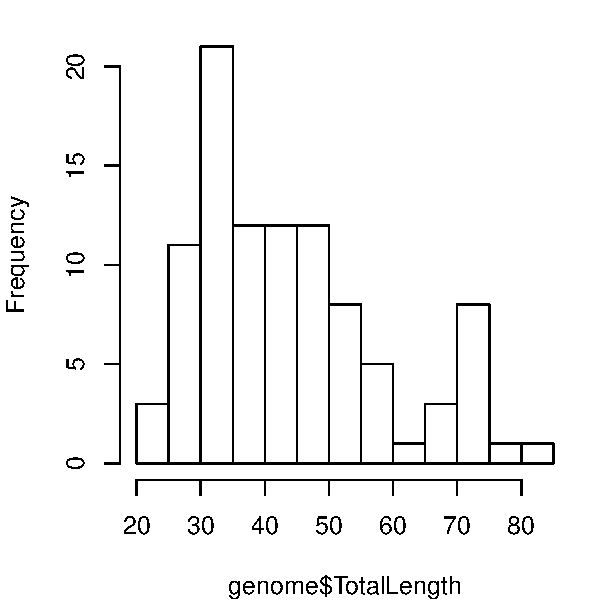
\includegraphics[width=0.45\textwidth]{histTL1}
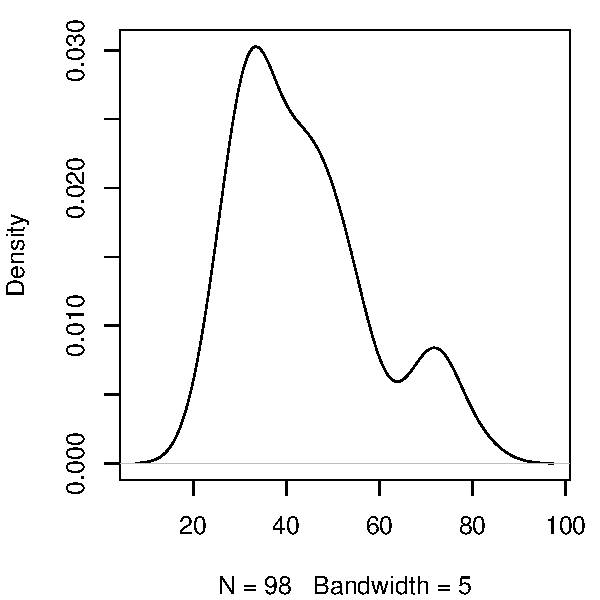
\includegraphics[width=0.45\textwidth]{histTL2} 
\end{center}
 
\subsection{Take a quick look at effects of certain factors}
R has a special way of describing a model that defines the response 
variable and the explanatory variables ("factors"). This is called a 
'formula' and is used to define linear models (more on these in a later 
chapters). The same structure is used in many plotting functions and 
will put the response variable on the $y$ axis and the explanatory 
variable on the $x$ axis. The structure is "response variable $\sim$ 
explanatory variables". We will look at multiple explanatory variables 
in a later practical but an example with one explantory variable 
(factor) is:

	{\tt Genome Size $\sim$ Suborder}

This formula tells R to model genome size `as a function of' 
($\sim$) the suborders of Odonata. In a plot function, the 
result will be to plot genome size as a function of the suborders.
 
\subsection{Compare distribution of the variable across levels of a 
factor}

Although looking at the distribution of variables is a good first step, 
we often want to compare distributions. In this case, we might want to 
know how genome size varies between dragonflies and damselflies. The 
first way we will look at is using boxplots --- these show the median 
and the 25\% and 75\% quantiles as a box, with whiskers extending to 
the minimum and maximum. More extreme outliers are plotted 
independently as points. The {\tt plot} function in R automatically 
generates a boxplot when the explanatory variable is a factor.

\begin{compactitem}[$\quad\star$]
\item Go to block 5 of the script and run the first line, looking at 
genome size between the two suborders.
\item Duplicate and alter this line to look at the same plot for total 
length. You should get a plot like this:
\end{compactitem}
 
\begin{center}
    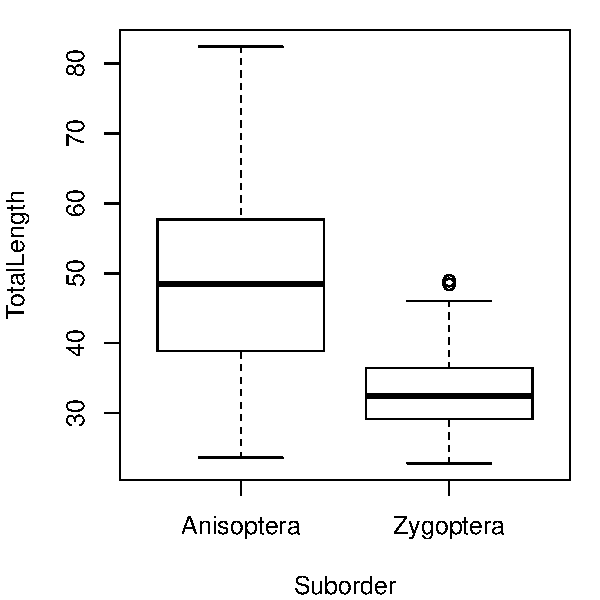
\includegraphics[width=0.55\textwidth]{bxpTL} 
\end{center}
 
Although histograms are great for one variable, plotting two histograms 
on top of one another rarely works well because the overlapping bars 
are hard to interpret (recall the predator-prey body size example). 
Density plots don't have this problem but it takes a bit more code to 
create the plot. 

\begin{compactitem}[$\quad\star$]
\item block 6 of the script uses the {\tt subset} function to create 
two new data frames separating the data for dragonflies and 
damselflies. Run the first two lines of this block. Remember that the 
arrow symbol ({\tt <-}) is used to save the output of a function into a 
new object in R --- if you use {\tt ls()} in the console, you will see 
the two new data frames.
\item In the console, use {\tt str} and {\tt summary} to explore these 
two new dataframes.
\end{compactitem}
Now that we've got the data separated we can go about plotting the two 
curves. 
\begin{compactitem}[$\quad\star$]
\item Run the next two lines of code in block 6. The first draws the 
plot for damselflies and the second adds a line for the dragonflies. 
\item Duplicate these last two lines of code and edit them to generate 
a similar plot for total body length. You will need to edit the code to 
change the range of the $x$ and $y$ axes ({\tt xlim} and {\tt ylim}) to 
get both curves to fit neatly on to the graph. It should look like 
this:
\end{compactitem}

\begin{center}
    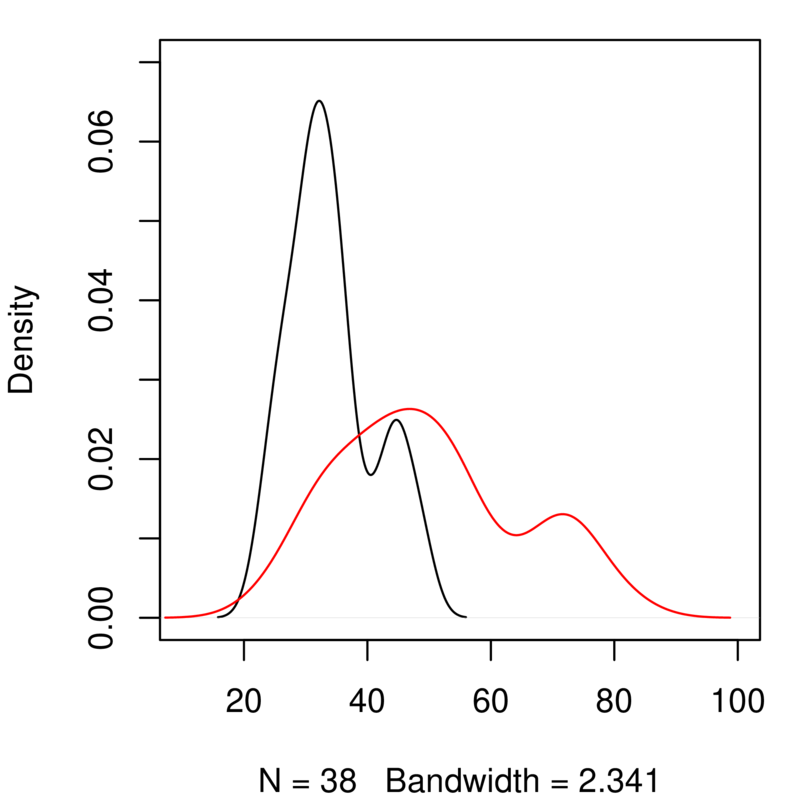
\includegraphics[width=0.45\textwidth]{densTL} 
\end{center}

\subsection{Explore further by scatter-plotting two variables}
 
Once we've looked at the distribution of variables, the next thing is 
to look at the relationships between continuous variables using 
scatterplots. The {\tt plot} function in R automatically generates a 
scatterplot when the explanatory variable is continuous, so we can use 
the same syntax and structure as for the boxplot above.
 
\begin{compactitem}[$\quad\star$]
\item Go to block (7) of the script and run the first plot command to 
plot body weight as a function of genome size.
\item Create a new line of code to plot forewing area as a function of 
genome size. It should look like this:
\end{compactitem}

\begin{center}
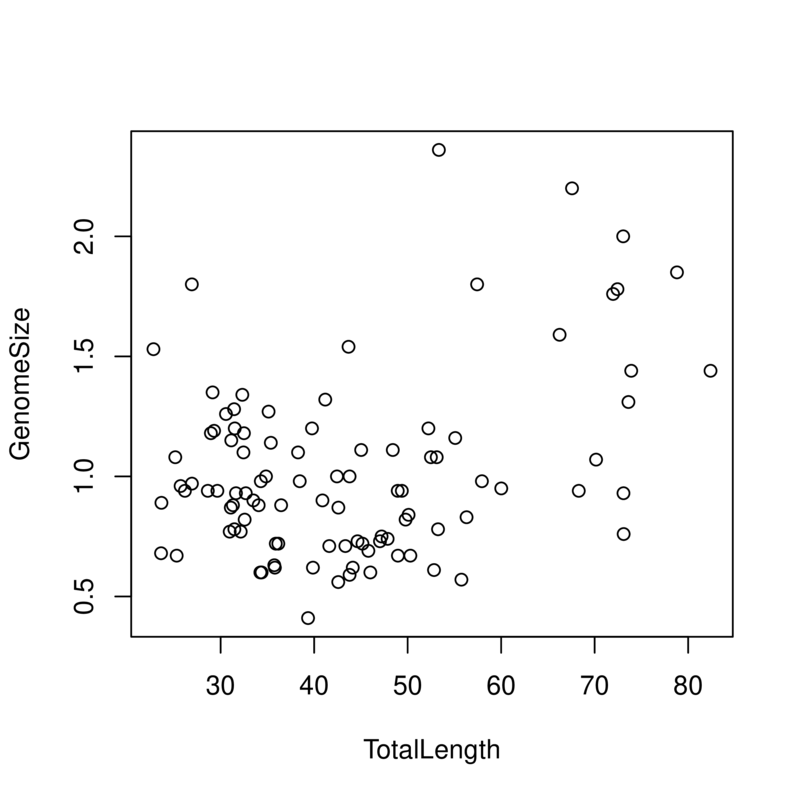
\includegraphics[width=0.5\textwidth]{scatWing} 
\end{center}
The scatterplot seems to show a weak relationship between 
genome size and morphology. But maybe dragonflies and damselflies show 
different relationships, and we can't distinguish between them! To 
explore this possibility, we need to plot the two orders using 
different colours or plot characters. In the next code block, we want 
customize the plots to show different types of points for each 
suborder. It is done by using {\it indexing} (covered in the first R Chapter in SilBioComp.pdf).

\begin{compactitem}[$\quad\star$]
\item Run the first two lines of code in block 8. There are two levels 
of suborder and these two lines set up a colour and a plot symbol that 
will be used for each one.
\item Run the next line which shows the structure of the factor {\tt 
Suborder}. You can see that there are two levels, with Anisoptera first 
and then Zygoptera. You can also see that these are stored as numeric 
values: 1 refers to the first level and 2 will refer to the second. We 
can use these as {\it indices} to pair the colours and plot symbols to 
each suborder. These are set in the {\tt plot} function using the 
options {\tt col=} and {\tt pch=}, which stands for "plot character".
\item Run the next plot command  to see the resulting plot --- each 
point gets the appropriate colour and symbol for its group.
\end{compactitem}
 
There are a lot of built in colours and plot symbols in R, so the next 
thing to experiment with is changing these to your own versions.

\begin{compactitem}[$\quad\star$]
\item In the console, type in the function {\tt colors()}. You'll see a 
long list of options to choose from, so pick two to replace red and 
blue in the script window.
\item The options for the plot symbols are shown below. Pick two to 
replace the current symbol choices.
\item Rerun the {\tt plot} function and see what you get!
\end{compactitem}

\begin{center}
    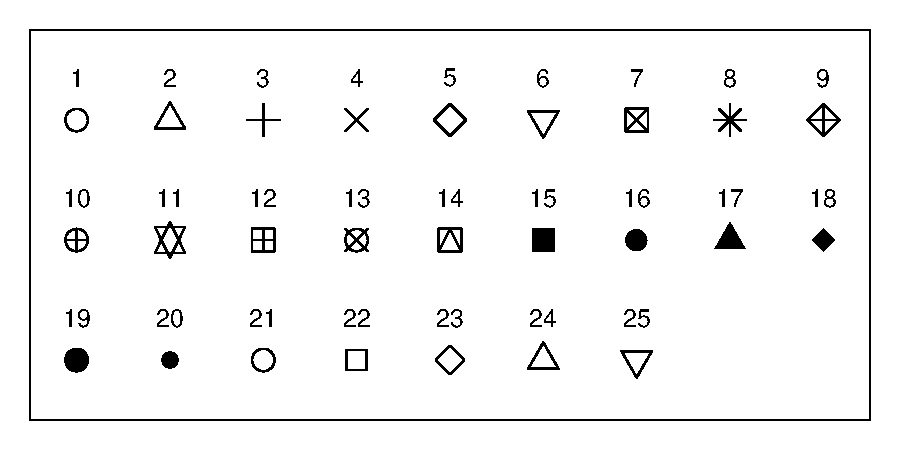
\includegraphics[width=0.55\textwidth]{pch} 
\end{center}
	
\subsection{Saving the exploratory graphics}
The file `GenomeSize.pdf' in the practical folder was created using the 
next block of code using the approach you learned previously. 
The function {\tt pdf} opens a new empty pdf file  which can then be 
used to plot graphs. You can set the width and the height of the page 
size in the pdf but note that this is set in {\it inches}. When you 
have finished creating a plot, the function {\tt dev.off} closes the 
pdf file and makes it readable.

\begin{compactitem}[$\quad\star$]
\item Open 'GenomeSize.pdf' in a PDF reader. It uses the original 
colours and plot symbols. Close the file and then delete it from the 
folder.
\item Now go back to the script in R and select and run all the code in 
block (9)
\item Go back to the {\tt Results} folder. The pdf file should have 
been recreated --- open it and it should now use your choice of colours 
and symbols.
\end{compactitem}

\subsection{Saving data}

One last thing you can do is to save the data and variables in R format 
--- the original data, two subsets of the data and the two sets of 
colours and symbols. We can recreate the subsets easily, so we'll just 
save the data and your colour sets.

\begin{compactitem}[$\quad\star$]
\item Go to the script window and run the final line in block (10)
\item Still in the script window, choose `File $\triangleright$ Save' 
to save your changes to the script file.
\item Quit from R {\tt q()}.
\end{compactitem}
